\documentclass[]{article}
\usepackage{graphicx}
\usepackage{float}
\usepackage{amsmath}
%\usepackage[]{hyperref}
% Title Page
\title{Lab 3}
\author{
	Alex Taglieri
	\\
	Andrew Kacherski
	}

\begin{document}
\maketitle
\newpage
\
\raggedright


\pagenumbering{arabic}
\section{Introduction and Background}

This lab shows the effects of damping on the mass-spring system we've been investigating in this course.

The general formula for the oscillation of a damped mass-spring system is given by the following equation:


\begin{equation}\label{uncertaintyLong}
x(t) = Ae^{\frac{-\gamma t}{2}}cos(\omega_d t + \phi)
\end{equation}

where $A$ is the amplitude, $\gamma$ is the damping ratio and can be found using the expression  $\gamma = \frac{b}{m}$ (where $b$ is the damping coefficient and $m$ is the mass), $t$ is time, $\omega_d$ is the damped frequency, and $\phi$ is the phase shift.

$\omega_d$ can be calculated using $k$, $m$, and $b$ (where $k$ is the spring constant):

\begin{equation}
	\omega_d = \sqrt{\frac{k}{m} - \frac{b^2}{4m^2}}
\end{equation}

It can also be determined using the variables $\omega_0$ and $\gamma$:

\begin{equation}
	\omega_d = \sqrt{\omega_0 ^2 - \frac{\gamma^2}{4}}
\end{equation}



\section{Procedure}

Hang two springs from the force sensor in series. Use varying masses between 100g and 400g to determine the k value of the two springs. 

Weigh the three disks of cardboard that should be around 5g, 10g, and 15g. Attach 400g to the hanging mass, and then add small masses until the mass of the hanging mass is 400g plus the weight of the heaviest mass. Zero the readings with the mass motionless, then set the mass in pure vertical oscillation a few centimeters in amplitude and record the results.
Now replace some of the small masses on the hanging mass with one of the cardboard disks, making sure that the overall mass of the system remains the same. Set the mass in motion once more. Repeat for each of the three cardboard disks.

\section{Results}

The springs in series had an overall \textit{k}-value of 16.33 N/m. The masses were within \textit{0.5g} of their expected mass.

The disks weighed 2.6g, 5g, and 13.4g for the small, medium, and large cardboard cutouts respectively.

The angular frequency observed for the undamped mass was 6.2595 rad/sec. When it was damped with the small disk, the new frequency was 6.278 rad/sec. For the medium disk the frequency was 6.253 rad/sec, and for the large disk the frequency decreased to 6.245 rad/sec.


\begin{figure}[H]
	\centering
	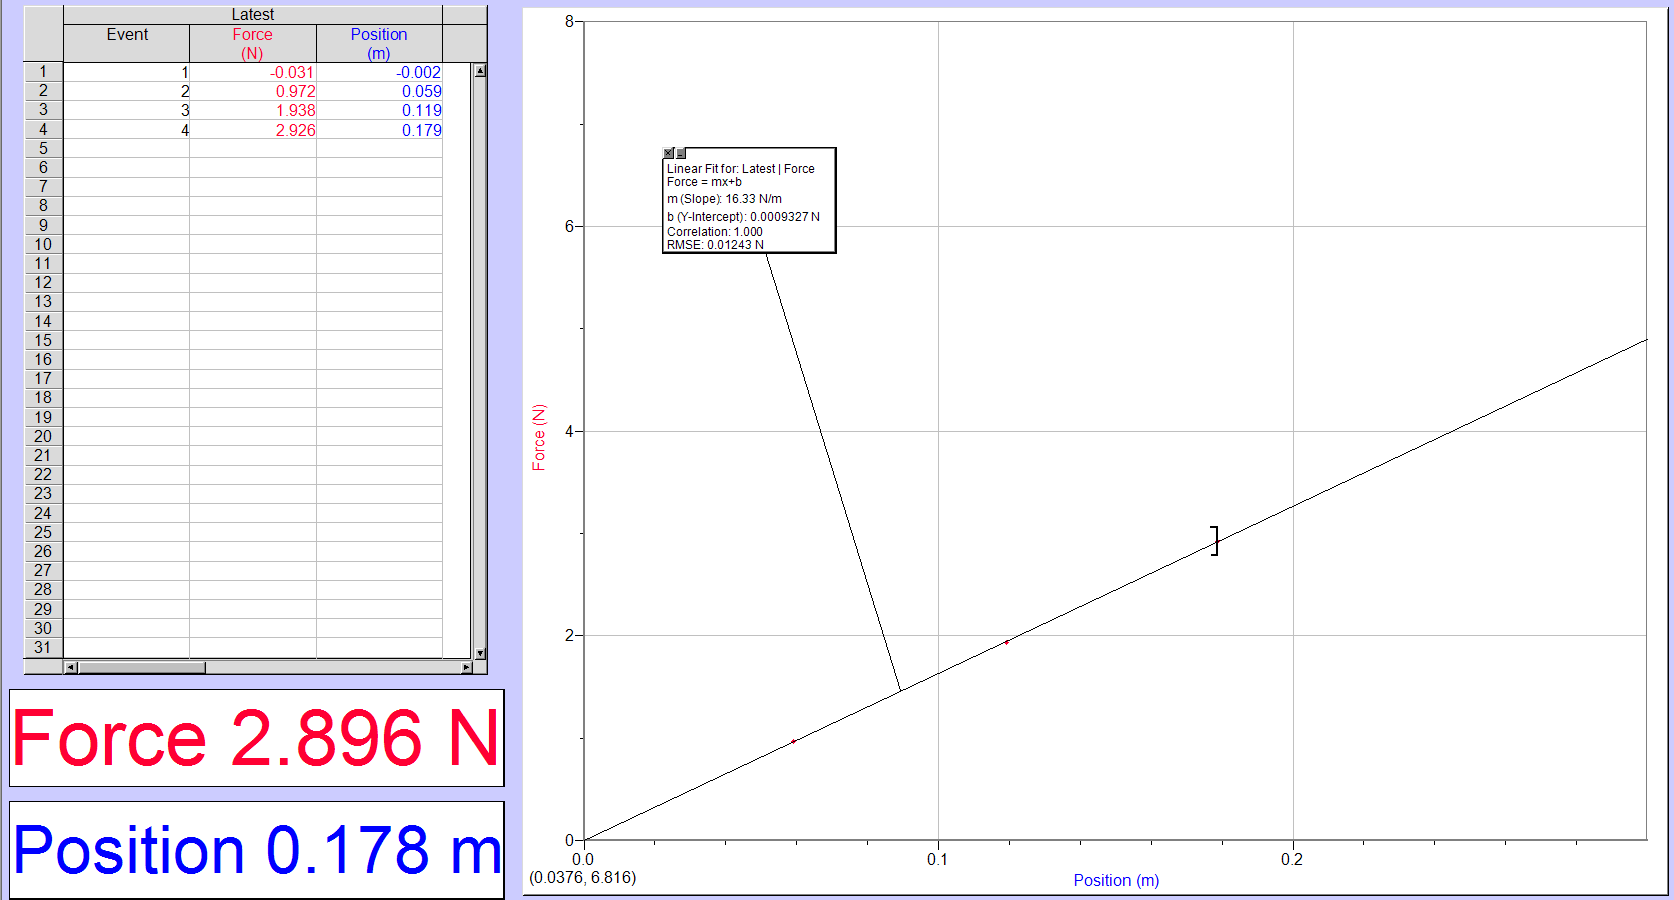
\includegraphics[width=\textwidth]{res/seriesSprings}
	\caption{Spring K Values}
	\label{fig:Spring K Values}
\end{figure}

\begin{figure}[H]
	\centering
	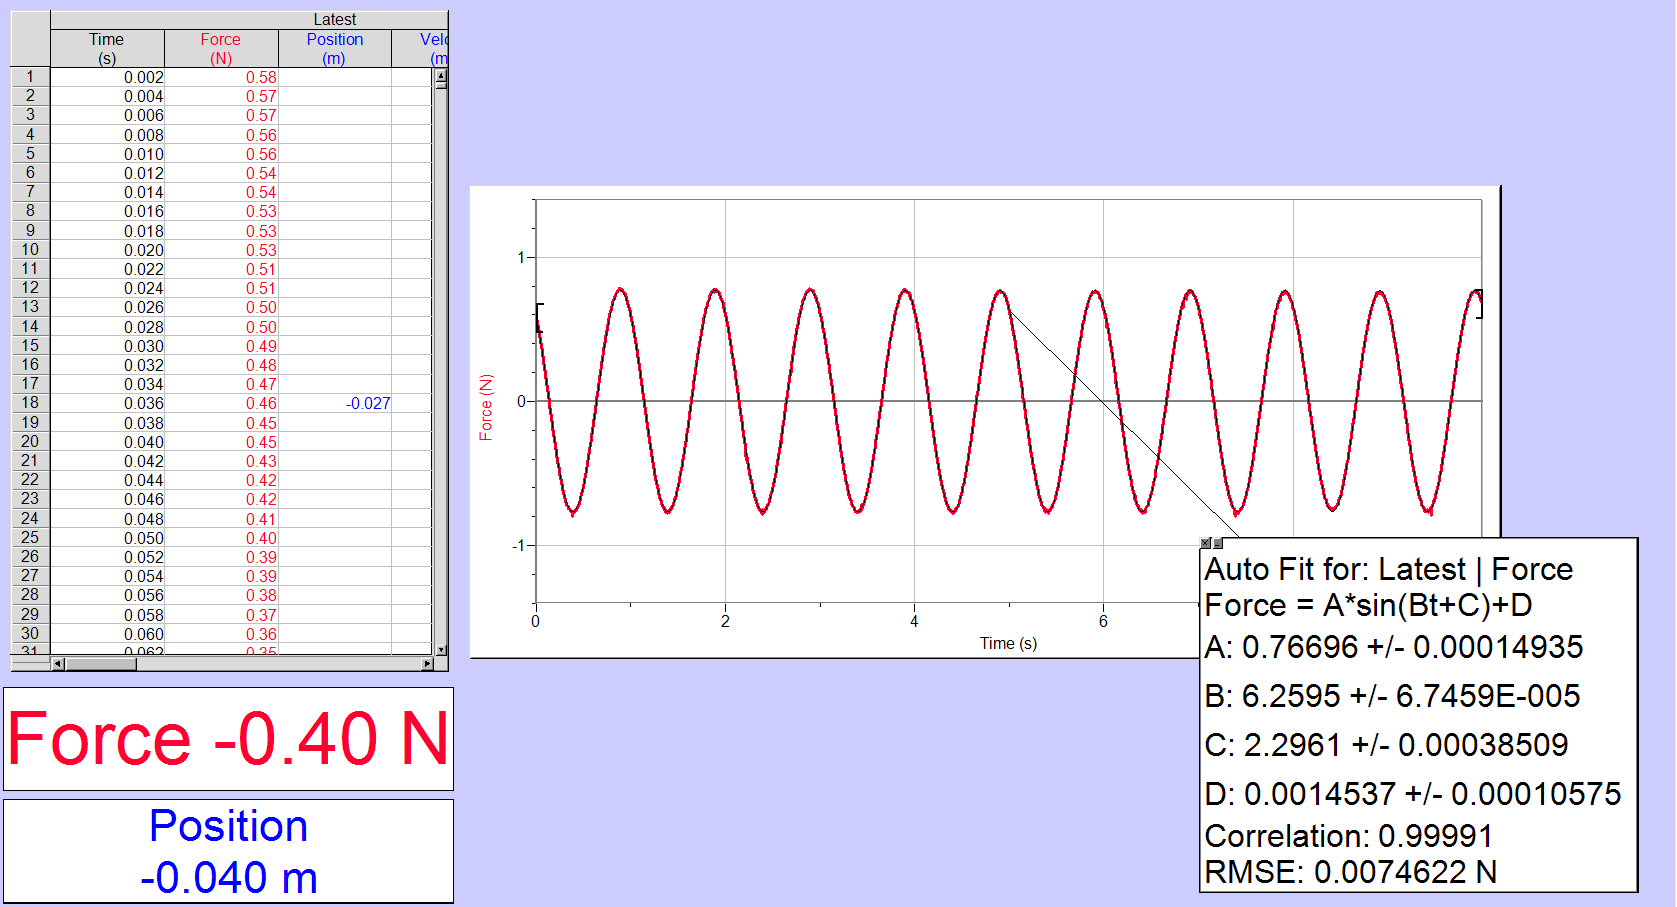
\includegraphics[width=\textwidth]{res/unDamped}
	\caption{Undamped Mass Oscillating}
	\label{fig:Spring K Values}
\end{figure}


\begin{figure}[H]
	\centering
	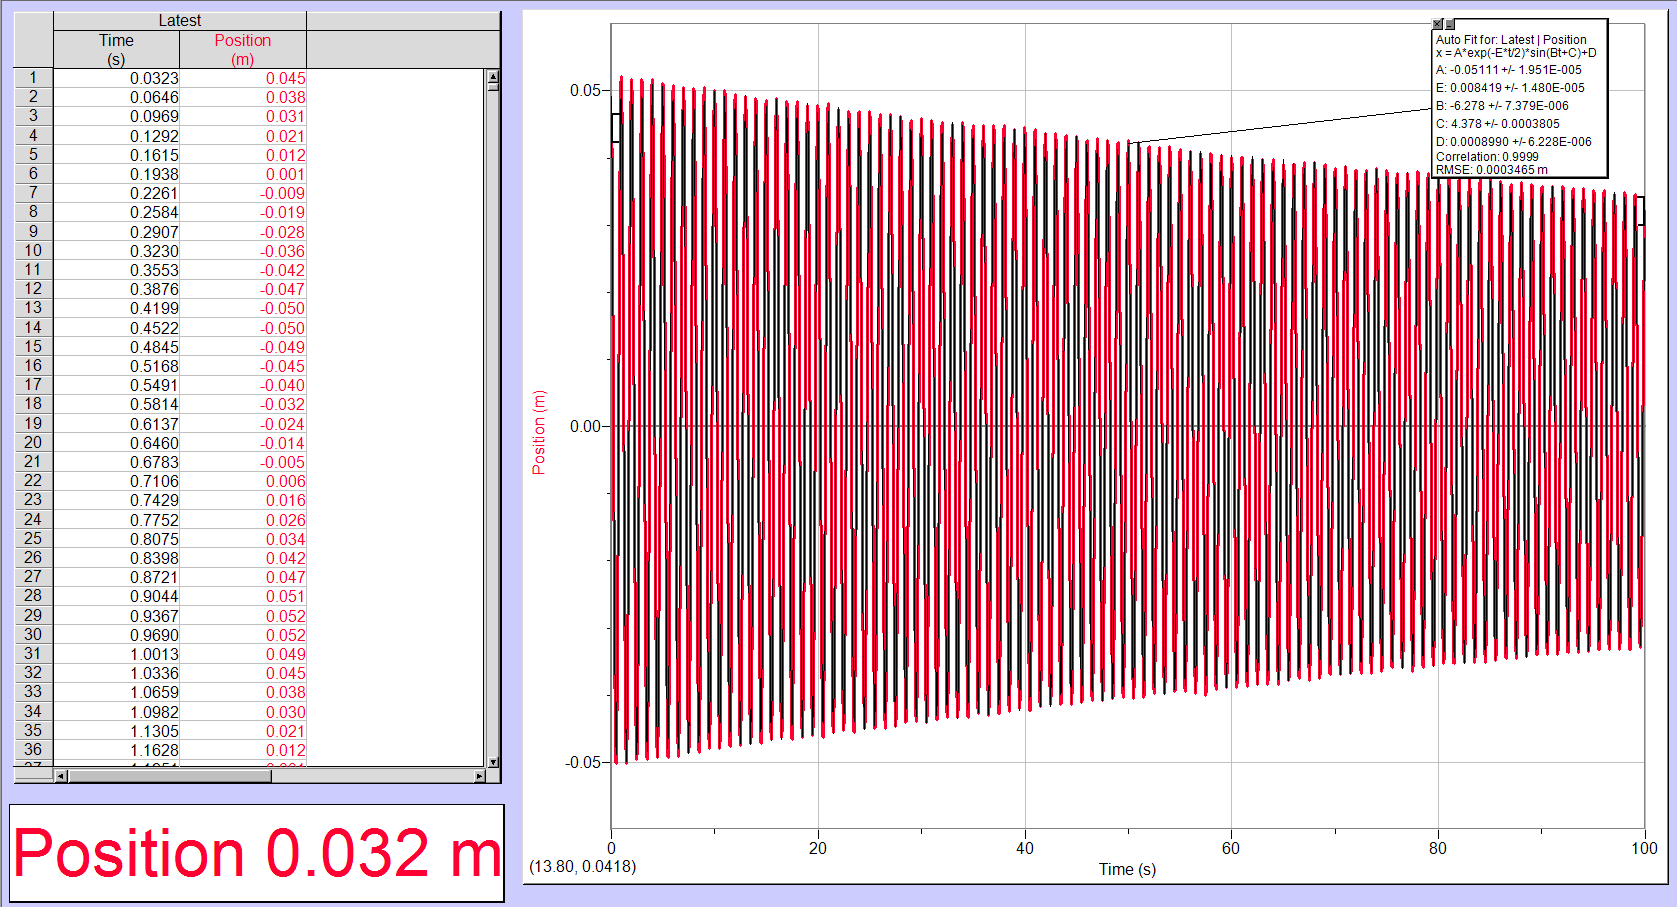
\includegraphics[width=\textwidth]{res/smallDamped}
	\caption{Mass with Small Damper}
	\label{fig:Mass with Small Damper}
\end{figure}

\begin{figure}[H]
	\centering
	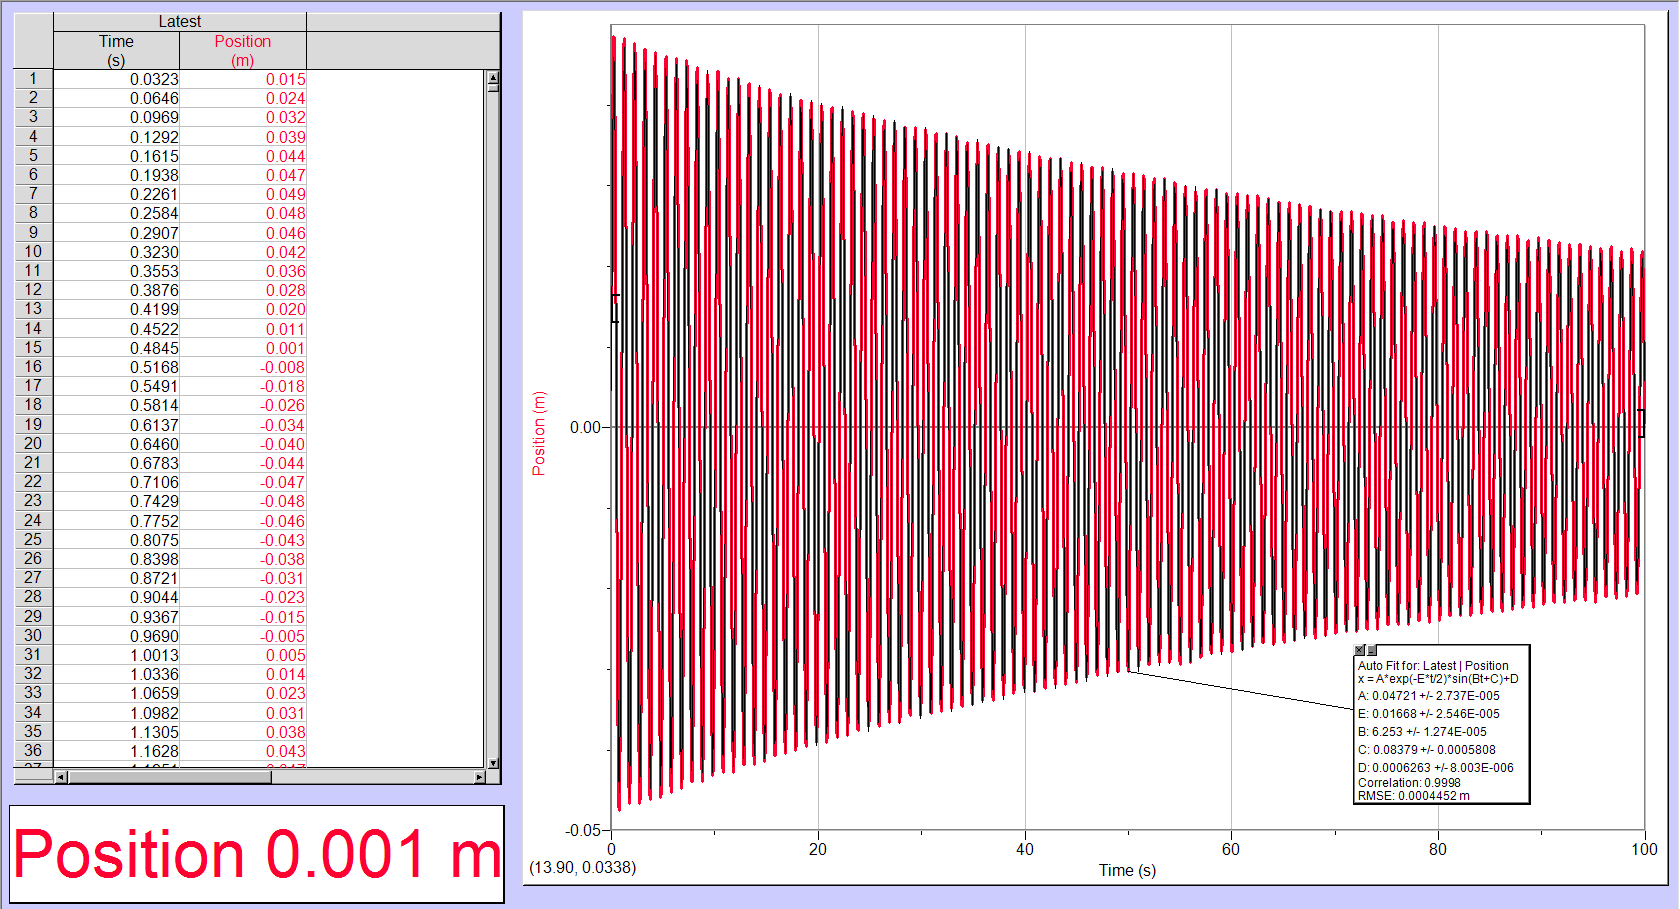
\includegraphics[width=\textwidth]{res/middleDamped}
	\caption{Mass with Medium Damper}
	\label{fig:Mass with Medium Damper}
\end{figure}

\begin{figure}[H]
	\centering
	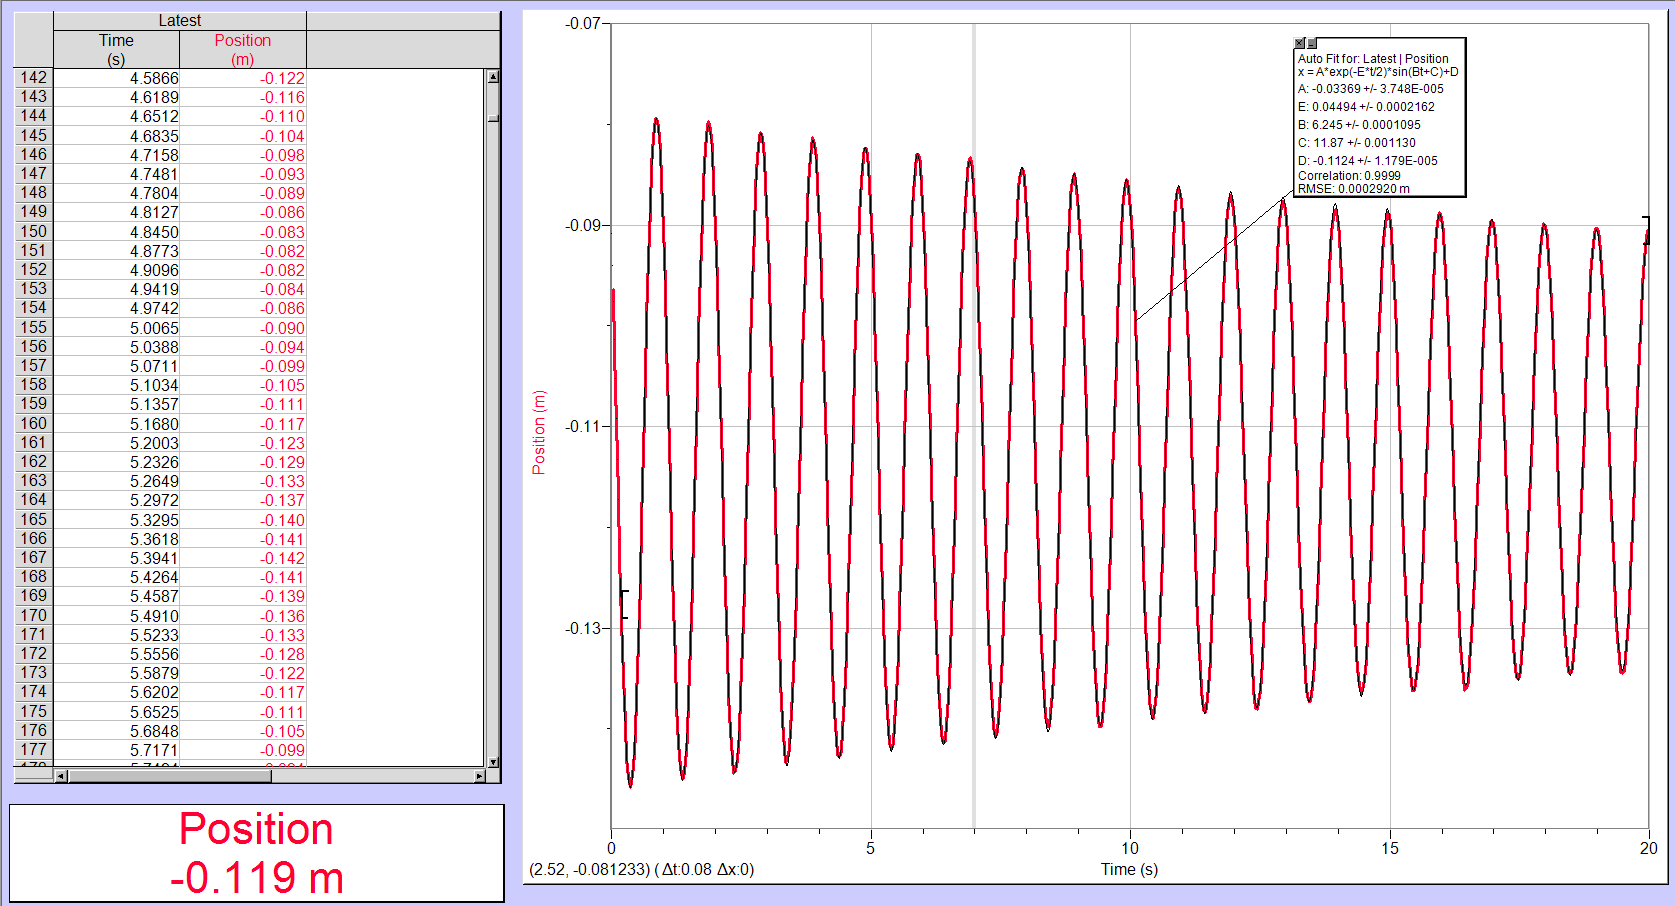
\includegraphics[width=\textwidth]{res/largeDamped}
	\caption{Mass with Large Damper}
	\label{fig:Mass with Large Damper}
\end{figure}



\section{Discussion}

In the Results section, we found the frequencies of oscillation of all four situations: small dampening disk, medium, large, and no dampening disk. Here we'll plug them into the equation from the Background section to predict what the damped frequencies should have been.

The equation from above is reproduced here:

\begin{equation}
\omega_d = \sqrt{\omega_0 ^2 - \frac{\gamma^2}{4}}
\end{equation}

For the small dampener, the $\gamma$ value was .00842, as calculated by Logger Pro. The equation above predicts that the damped frequency should be $\sqrt{6.2595^2 - \frac{.00842^2}{4}} = 6.2595$ rad/sec (The damped frequency and the undamped one are actually slightly different, but rounding brings the numbers back to nearly the same value). The medium damped frequency should be $\sqrt{6.2595^2 - \frac{.01668^2}{4}} = 6.2595$ rad/sec (Once again, the damped frequency is slightly below the undamped frequency but the actual value is hidden by a rounding error), and the experiment with the large disk's damped frequency should have been $\sqrt{6.2595^2 - \frac{.04494^2}{4}} = 6.25946$ rad/sec (The difference between the damped and undamped frequencies is now visible but still mostly negligible).

The dampening coefficient of the medium disk (.01668) was twice that of the small disk (.00842), and the dampening coefficient of the large disk (.04494) was a little more than twice that of the medium disk. Their diameters roughly doubled from each size to the next, so this relationship makes sense.


In all of our equations we are assuming that we're calculating the coefficient \textit{b} from the equation $m \frac{d^2 x}{dt^2} + b \frac{dx}{dt} + kx = 0$, but that's not quite true. Air is a compressible fluid, and the drag force on an object moving through air is proportional to the square of its speed: 

\begin{equation}
F_d = \frac{C_d * \rho * v^2 * A}{2}
\end{equation}


 where $F_d$ is the force of drag, $C_d$ is the drag coefficient, $\rho$ is the density of the fluid, $v$ is the speed, and $A$ is the area. However, at the velocities involved in this lab, $v^2 \approx v$.


A possible source of error for all these calculations is that when we measured values for the undamped system the mass was 415g, but when the system was damped the mass was only 413g. The lowest resolution of masses that we had was 5g.


\end{document}          
